\section{Implementation}

\subsection{About Ngene}
Ngene is a generic, multipurpose genetic algorithm written in C++ with heavy focus on performance. The engine is divided into logical modules that can be interchanged or extended upon in order to fit the intended goal and purpose, all without the need to recompile a single line of code.

\subsubsection{Design}
The program is broken into the following modules:

\begin{itemize}
	\item (core) - The genetic algorithm itself
	\item Fitness - Assesses the fitness of a genotype
	\item Genotype - Produces the genotype and translates them to phenotype
	\item Mating - Crosses two genotypes
	\item Mutator - Mutates a genotype
	\item Selector - Selects a random genotype
\end{itemize}

The purpose of this is, as mentioned earlier, to make it more flexible with regards to the use of different modules with different experiments. For example, I used the \emph{tournament} selection module for most of the experiments I did on this thesis. I didn't have to recompile the same piece of code everytime I made a change in, say, the genotype module. This keeps the code cleaner and easier to maintain as well as it cuts down on the compilation time.

A problem with writing a generic genetic algorithm in a strongly typed programming language as C++, is that different studies require different datatypes to be passed around the system. A simple program that sorts numbers, for instance, needs to pass around an array with integers while another one may require the use of a class or custom datatype. In a higher level language such as Python, a container is already available that can store any type of data:

\begin{verbatim}
>>> foo = 1
>>> print foo
>>> foo = "awesome"
>>> print foo
awesome
>>> _
\end{verbatim}

Such a container is unfortunately not readily available in C++ and must be implemented in order for the modular design to work. Fortunately, this has already been done and is freely available as part of \emph{Boost C++ Libraries}\footnote{http://www.boost.org/}. \emph{Boost.Any}\cite{henney2001} is a container not very different from the one found in Python and only requires a type-casting before the data can be handled the normal way.

\subsubsection{Brief System Overview}
\begin{figure}[ht]
	\centering
	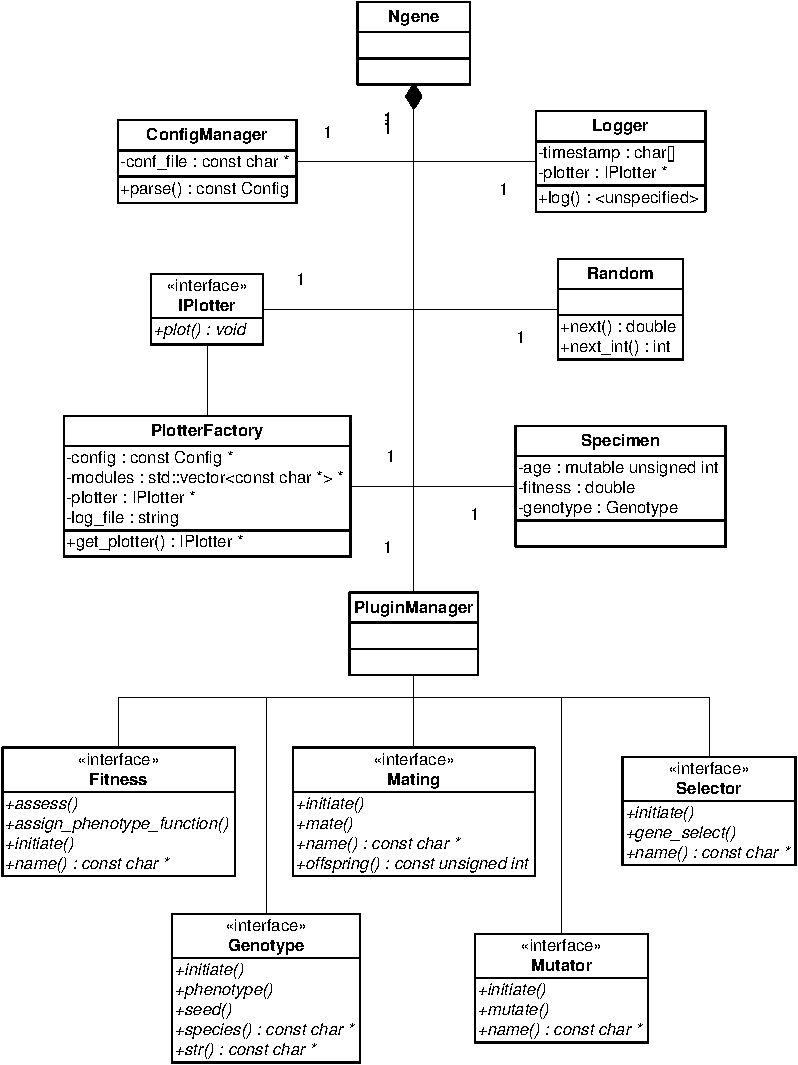
\includegraphics[scale=0.8]{diagram_ngene}
	\caption{Overview of Ngene}
	\label{fig:diagram_ngene}
\end{figure}

Figure~\ref{fig:diagram_ngene} shows a brief overview of how Ngene is put together.

When the program starts up, \texttt{Ngene} will pass on any parameters to the \texttt{ConfigManager}, which will start parsing the configuration file, and then pass on the parsed configuration to the \texttt{PluginManager}.

The \texttt{PluginManager} handles all loading and unloading of the modules specified in a configuration file. It also acts as an interface for the engine to communicate with the modules. The advantage of doing it this way, is that it enables swapping of modules without the need to recompile the whole code. The \texttt{PluginManager} will automatically unload all loaded modules when it is destroyed on program exit.

Next, the \texttt{Logger} is instantiated. This class makes sure that it has writing access in order to output the best specimen and plot a graph of the whole process. What the \texttt{Logger} should output is left to the author of the \texttt{Genotype} module and could be anything from a simple text file to a proprietary file format. The \texttt{Plotter} currently only supports SVG\footnote{Scalable Vector Graphics - http://www.w3.org/Graphics/SVG/}.

Finally, the engine will start producing random genotypes, or \texttt{Specimen}s, before starting the evolution. This process ends when a perfect \texttt{Specimen} is found, e.g. \texttt{fitness = 1.0}, or the number of generations has been reached. The \texttt{Logger} will then produce twofiles, and the program exits.

\texttt{Ngene} talks with its modules via pre-defined interfaces. All modules must implement these in order to be compatible with \texttt{Ngene}. A more detailed description and sample code can be found in the system documentation. Besides these restrictions, a user can extend the system in any way they see fit.


\subsection{Ngene Development Framework}
\begin{figure}[ht]
	\centering
	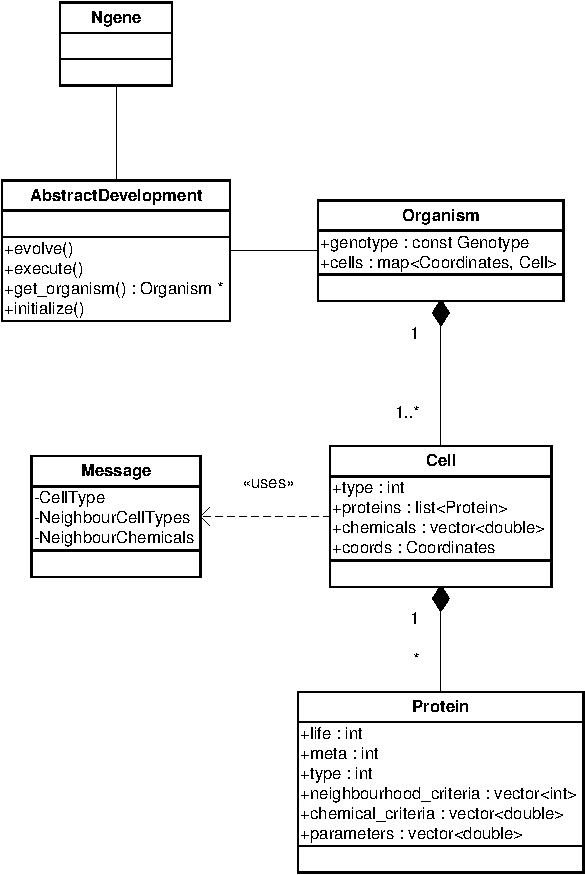
\includegraphics[scale=0.8]{diagram_ndevframe}
	\caption{Overview of Ngene Development Framework}
	\label{fig:diagram_ndevframe}
\end{figure}

To further extend the genetic algorithm already implemented in \emph{Ngene}, a generic development framework has also been put into place. This framework consists of an abstract class that must be implemented and a few pre-defined classes that the user may choose to use (see fig.~\ref{fig:diagram_ndevframe}). However, when comparing two development models, it is best to use as much common code as possible to eliminate more hidden factors. A common \texttt{Message} class is also available for information exchange between all \texttt{Cell}s (see fig.~\ref{fig:diagram_ndevframe_msg}).

\begin{figure}[ht]
	\centering
	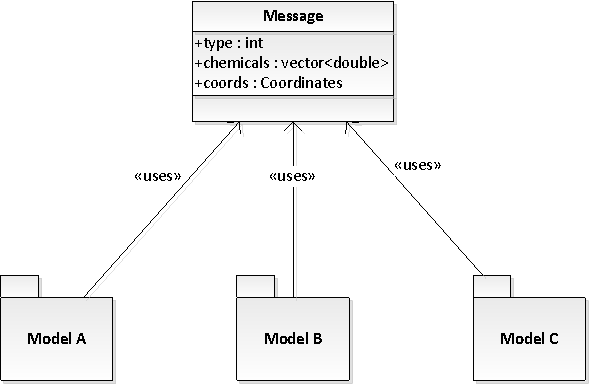
\includegraphics[scale=0.8]{diagram_ndevframe_msg}
	\caption{A common message implementation should eliminate some factors involving what information is exchanged between the organism's cells.}
	\label{fig:diagram_ndevframe_msg}
\end{figure}

A module can be created by inheriting \texttt{AbstractDevelopment} and implementing the required methods, \texttt{execute()} and \texttt{initialize()}. The latter is executed everytime a new organism is to be developed, while the former function is run every tick (see fig.~\ref{fig:diagram_ndevframe_ex}). 

\begin{figure}[ht]
	\centering
	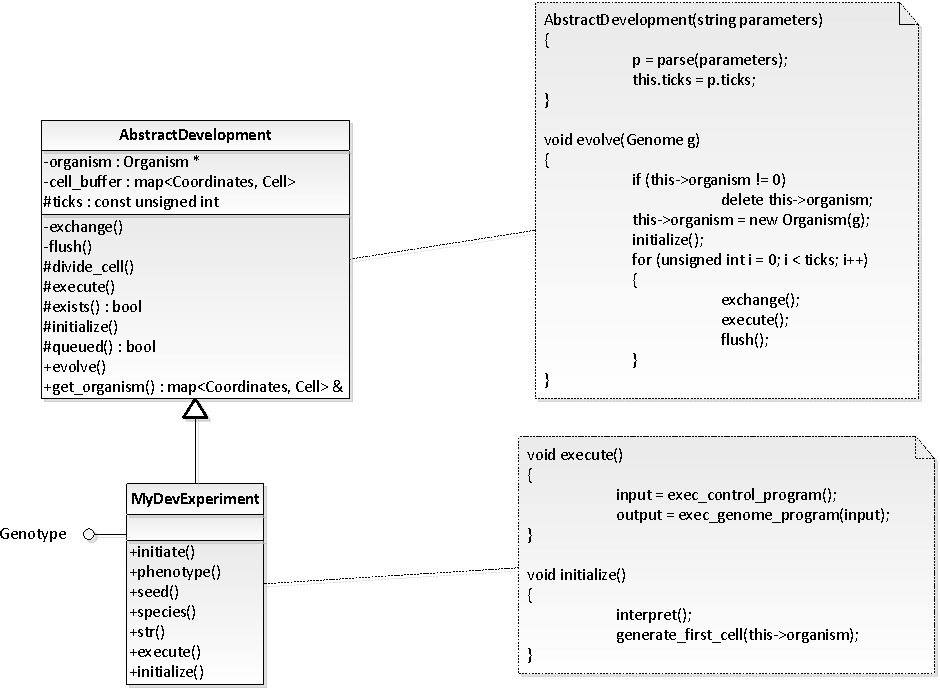
\includegraphics[scale=0.8]{diagram_ndevframe_ex}
	\caption{It's awesome.}
	\label{fig:diagram_ndevframe_ex}
\end{figure}


\subsubsection{Johan H{\o}ye's Model}
Based on Johan H{\o}ye's master's thesis\cite{hoye2006}, his model has been ported to this new framework.


\subsubsection{Julian F. Miller's Model}
This model is based a number of works such as \cite{ecal2003}.
